\documentclass[../main.tex]{subfiles}

\begin{document}
    \section{Mathematics behind Deep Neural Network}
        \subsection{Neural Network}
            \textbf{Neural network} is the core concept in deep learning. It's a network-like structure that tries to imitate human's neural system.
            A neural network consists of tons of numbers, we call each number a  \textbf{neuron}.
            A neural network can be split into \textbf{layers}: a smaller structure that also consists of neurons.
            As you can see in the following image that there are rectangles have circles in them. These rectangles are layers and circles are neurons.
            Those arrows between neurons/layers are \textbf{connections}. Connections stand for some kind of computations between neurons(numbers).
            \begin{note}
                A \textbf{Neural network} is just a structure that defines a specific connection among neurons.\\
                \textbf{Layer} is a smaller structure that help us construct, understand and explain a neural network.\\
                \textbf{A neural network consists of layers. A layer consists of neurons. Neurons are just numbers. Connections between neurons are some kind of computations.}
            \end{note}
            
            \begin{figure}[h]
                    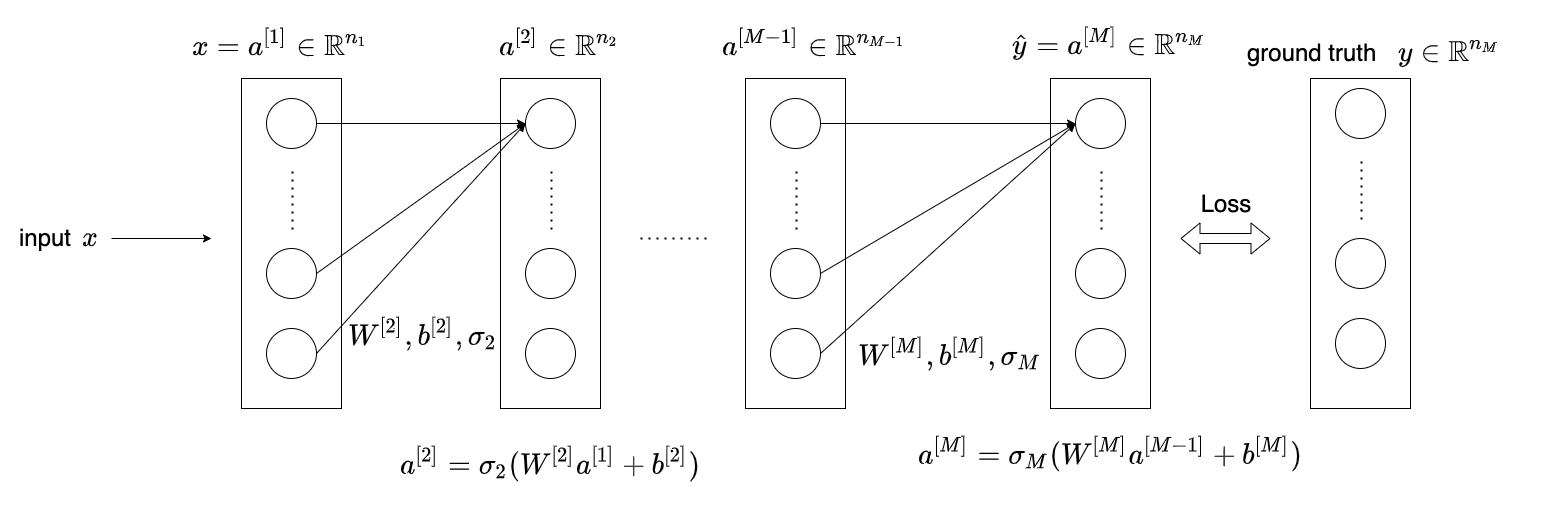
\includegraphics[width=\textwidth]{DNN.png}
                    \centering
            \end{figure}
            
            To construct a neural network, construct layers first.
            Each layer can be regarded as a real vector.
            In the image above, the first layer is $a^{[1]}$, it's a real vector has $n_1$ dimension; the second layer is $a^{[2]}$, a real vector has $n_2$ dimension, and so on, where each $n_i \in \mathbb{N}$.
            
            Second, we make connections among layers.
            Because layers are regarded as vectors, it's quite intuitive to define connections between them by matrix computation.
             
            For example, in the above image, the connection between the first two layers, $a^{[1]}$ and $a^{[2]}$, can be defined by a matrix $W^{[2]}$, a bias vector $b^{[2]}$ and an activation function $\sigma_2$. That is,
            \[
                a^{[2]} = \sigma_2(W^{[2]} a^{[1]} + b^{[2]})
            \]
            where $W^{[2]} \in \mathbb{R}^{n_2 \times n_1}$, $b^{[2]} \in \mathbb{R}^{n_2}$ and $\sigma_2: \mathbb{R}^{n_2} \rightarrow \mathbb{R}^{n_2}$.
            
            After finishing the construction of all connections, we can put our data $x$ into this neural network, $x$ will go through all these connections and output a vector $\hat{y}=a^{[M]}$.
            This process is called \textbf{feed forward}, \textbf{predict} or \textbf{inference}. Though this structure is quite complex, we can just interpret a neural network as a vector function $f$ that
            \[ 
                f:\mathbb{R}^{n_1} \rightarrow \mathbb{R}^{n_M}
            \]
            
            The goal of a neural network is predicting a vector $\hat{y}$ that almost the same as a predefined ground truth $y$.
            When $\hat{y}$ is way more different from $y$, we need a mechanism to let this network correct all the connections to let $\hat{y}$ look more alike to $y$.
            So here comes the loss function, the double arrow in the picture. It's a function that compare how similar $\hat{y}$ and $y$ are.
            In general, we'll choose a function that take two vectors as input and a non negative number as output, and then \textbf{define these two vectors are similar when the output number closes to} $0$.(For example, the well known L2 norm $\|\hat{y} - y\|_2$.)
            That is to say, the mechanism need to let the network try its best to lower down the value of the loss function(by adjusting the connection), then its output $\hat{y}$ will look like the ground truth $y$. 
            
            In reality, there won't be only one $(x, y)$ pair. When we have lots of training data $\{(x_i, y_i)\}_1^n$, we'll give a neural network lots of example to follow up: 
            \begin{displayquote}
                Input $x_1$, output $\hat{y}_1$, adjust the connection to fit $\hat{y}_1$ to $y_1$; Input $x_2$, output $\hat{y}_2$, adjust the connection to fit $\hat{y}_2$ to $y_2$; Input $x_3$, output $\hat{y}_3$, adjust the connection to fit $\hat{y}_3$ to $y_3$, ...
            \end{displayquote}
            
            This mechanism is so called \textbf{training a neural network} and we use a method called \textbf{back propagation} to achieve training.
            
            We need to set up some notations to explain the details of how back propagation works.
            
        \subsection{Notations}
            Assume there are $M$ layers.
            The $k^\mathrm{th}$ layer will has $n_k$ neurons and is denoted by a vector $a^{ [k] }\in \mathbb{R}^{n_k}$.
            The matrix, bias vector and the activation function between the $k-1^{\mathrm{th}}$ layer and the $k^\mathrm{th}$ layer are denoted by $W^{ [k] }\in \mathbb{R}^{ n_k\times n_{k-1} }$, $b^{[k]} \in \mathbb{R}^{n_k}$ and $\sigma_k: \mathbb{R}^{n_k} \rightarrow \mathbb{R}^{n_k}$, respectively, where $k=2,\dots,M$.
            To simplify the computation, we let the activation functions are all the same as the function $\sigma(x) = \frac{1}{1+e^{-x}}$ and note that
            \[
                \sigma(x) = \left( 
                    \begin{array}{c}
                        \frac{1}{1+e^{-x_1}} \\
                        \frac{1}{1+e^{-x_2}} \\
                        \vdots \\
                        \frac{1}{1+e^{-x_n}}                         
                    \end{array}
                \right),\quad\mathrm{for~}x=\left(
                    \begin{array}{c}
                        x_1 \\
                        x_2 \\
                        \vdots \\
                        x_n
                    \end{array}
                \right) \in \mathbb{R}^n
            \]
            
            Let $\{(x_i, y_i)\}_1^n$ be our training data, then the feed forward process can be formalized as 
            \begin{align*}
                & a_i^{ [1] } = x_i \in \mathbb{R}^{n_1}, \\
                & a_i^{ [2] } = \sigma (W^{ [2] }a_i^{ [1] } + b^{ [2] }) \in \mathbb{R}^{n_2}, \\
                & a_i^{ [3] } = \sigma (W^{ [3] }a_i^{ [2] } + b^{ [3] }) \in \mathbb{R}^{n_3}, \\
                & \qquad\vdots\\
                & a_i^{ [k] } = \sigma (W^{ [k] } a_i^{ [k-1] } + b^{ [k] }) \in \mathbb{R}^{n_k}, \\
                & \qquad\vdots\\
                & a_i^{ [M] } = \sigma (W^{ [M] } a_i^{ [M-1] } + b^{ [M] })=\hat{y}_i \in \mathbb{R}^{n_M}
            \end{align*}
            
            We need to let neural network know what "closeness of two vectors" actually mean. Let's defined a loss function that take $\hat{y}_i$ and $y_i$ as input and a non negative number as output:
            \[
                L(\hat{y}_i, y_i)=\frac{1}{2}\left\|\hat{y}_i - y_i\right\|_2^2
            \]
            When $L(\hat{y}_i,y_i) \rightarrow 0$, we consider $\hat{y}_i$ and $y_i$ are similar at neural network's aspect.
            
            You may wonder why we choose L2 norm rather than other function. The answer is:
            \begin{displayquote}
                There's no best solution of how to choose a loss function, you need lots of experiment and paper reading to hone your intuition.
            \end{displayquote}
            
        \subsection{*Training}
            \[
                \sum_{i=1}^nL(a_i^{[M]}, y)=\sum_{i=1}^n\frac{1}{2}\left\|a_i^{[M]} - y_i\right\|_2^2
            \]
            The recursive relations of each $a^{[i]}$ shows that the loss function actually depends on all the matrices $W^{[i]}$, all the bias vectors $b^{[i]}$ and the ground truth $y$
            \[
                L(W^{ [2] }, W^{ [3] },\dots,W^{[M]},b^{[2]},b^{[3]},\dots,b^{[M]}, y)=\frac{1}{2}\left\|y-a^{[M]}\right\|_2^2
            \]
            We can ignore $y$ here since it's a constant in the computation, so
            \[
                L(W^{ [2] }, W^{ [3] },\dots,W^{[M]},b^{[2]},b^{[3]},\dots,b^{[M]})=\frac{1}{2}\left\|y-a^{[M]}\right\|_2^2
            \]
            
            Now our goal is finding each  $W^{[k]}$ and $b^{[k]}$ to let $a^{[M]}$ be closer to $y$.
            This is what training means in mathematics.
 
            Let $\theta=(W^{[2]},\cdots,W^{[M]},b^{[2]},\cdots,b^{[M]})$, then $\theta\in\mathbb{R}^D$, where
            \[
                D = \sum_{k=2}^M n_k\times n_{k-1}+\sum_{k=2}^M n_k
            \]
            Then the training problem becomes like this
            \[
                \argmin_\theta \left\|y - a^{[M]}\right\|_2^2\equiv\argmin_\theta L(\theta)
            \]
            where $L:\mathbb{R}^D \rightarrow \mathbb{R}$. 

        \subsection{Main Computations}
            To compute $\nabla L(\theta)$. Let $z^{ [k] } = W^{ [k] } a^{ [k-1] } + b^{ [k] }$ then $a^{ [k] } = \sigma(z^{ [k] })$.
            Let $j$ be the index represents neurons of each layer. The notation becomes
            \begin{align*}
                & z_j^{[k]}=(W^{[k]}a^{[k-1]}+b^{[k]})_j=(W^{[k]}a^{[k-1]})_j+b_j^{[k]}, \\
                & a_j^{[k]}=\sigma(z^{[k]})_j, \\
                & k=2,\dots,M,\quad j=1,\dots,n_k
            \end{align*}
            The core concept of back propagation is using deep level derivatives to compute shallow level derivative. This can be achieved with the help of chain rule. First we derive the derivative of $z^{[k]}_j$(the $j^\mathrm{th}$ neuron of the $k^\mathrm{th}$ layer).
            \begin{align*}
                & \frac{\partial L(\theta)}{\partial z_j^{[M]}} = \frac{\partial L(\theta)}{\partial a_j^{[M]}}\frac{\partial a_j^{[M]}}{\partial z_j^{[M]}}=\frac{\partial L(\theta)}{\partial a_j^{[M]}}\sigma'(z_j^{[M]})=(a_j^{[M]}-y_j)\sigma'(z_j^{[M]})=(a_j^{[M]}-y_j)a_j^{[M]}(1-a_j^{[M]}), \\
                & \frac{\partial L(\theta)}{\partial z_j^{[M-1]}} = \frac{\partial}{\partial z_j^{[M-1]}}\frac{1}{2}\sum_{k=1}^{n_M}\Big(y_k-\sigma\big(W^{[M]}\sigma(z^{[M-1]}) +b^{[M]}\big)_k\Big)^2 \\
                & \phantom{\frac{\partial L(\theta)}{\partial z_j^{[M-1]}}} =\nabla_{z^{[M]}}L(\theta)\cdot\frac{\partial z^{[M]}}{\partial z_j^{[M-1]}} \\
                & \phantom{\frac{\partial L(\theta)}{\partial z_j^{[M-1]}}} = \sum_{m=1}^{n_M} \frac{\partial L(\theta)}{\partial z_m^{[M]}}\frac{\partial z_m^{[M]}}{\partial z_j^{[M-1]}} \\
                & \phantom{\frac{\partial L(\theta)}{\partial z_j^{[M-1]}}} = \sum_{m=1}^{n_M} \frac{\partial L(\theta)}{\partial z_m^{[M]}}\left(\frac{\partial}{\partial z_j^{[M-1]}}\sum_{s=1}^{n_{M-1}}w_{ms}^{[M]}\sigma(z_s^{[M-1]})+b_m^{[M]}\right) \\
                & \phantom{\frac{\partial L(\theta)}{\partial z_j^{[M-1]}}} = \sum_{m=1}^{n_M} \frac{\partial L(\theta)}{\partial z_m^{[M]}}w_{mj}^{[M]}\sigma'(z_j^{[M-1]}) \\
                & \phantom{\frac{\partial L(\theta)}{\partial z_j^{[M-1]}}} = \sigma'(z_j^{[M-1]})\left((W^{[M]})^T\frac{\partial L(\theta)}{\partial z^{[M]}}\right)_j \\
                & \phantom{\frac{\partial L(\theta)}{\partial z_j^{[M-1]}}} = \left((W^{[M]})^T\frac{\partial L(\theta)}{\partial z^{[M]}}\right)_ja_j^{[M-1]}(1-a_j^{[M-1]}), \\
                & \qquad\qquad\qquad\vdots \\
                & \frac{\partial L(\theta)}{\partial z_j^{[1]}} = \left((W^{[2]})^T\frac{\partial L(\theta)}{\partial z^{[2]}}\right)_ja_j^{[1]}(1-a_j^{[1]})
            \end{align*}
            From above we can see that we \textit{back propagate} the derivative since we need $\partial z^{[M]}$ to yield $\partial z^{[M-1]}_j$. The partial derivative of $z_j^{[k]}$ can help us get the gradient w.r.t weight and bias.
            \begin{align*}
                & \frac{\partial L(\theta)}{\partial b_j^{[k]}}=\frac{\partial L(\theta)}{\partial z_j^{[k]}}\frac{\partial z_j^{[k]}}{\partial b_j^{[k]}}=\frac{\partial L(\theta)}{\partial z_j^{[k]}}, \\
                & \frac{\partial L(\theta)}{\partial w_{js}^{[k]}}=\frac{\partial L(\theta)}{\partial z_j^{[k]}}\frac{\partial z_j^{[k]}}{\partial w_{js}^{[k]}}=\frac{\partial L(\theta)}{\partial z_j^{[k]}}a_s^{[k]}
            \end{align*}
            And hence we can back propagate each $\partial b^{[k]}_j$ and $\partial w^{[k]}_{js}$.

            For the case with multiple training instances $(x_i, y_i)$, $i=1,\dots,N$. The loss function becomes
            \[
                L(\theta) = \frac{1}{N} \sum_{i=1}^N \frac{1}{2} \|y_i - a_i^{[ [M] }\|_2^2    
            \]
            The computation are all the same but the notation will become a little bit complicated.
\end{document}
    